%
%  Scott Percic
%
\documentclass[12pt,fullpage]{article}
\usepackage{fullpage}
\usepackage{psfrag}                                          % LaTeX graphics tool
\usepackage{pslatex}                                         % avoids the default cmr font
\usepackage{graphicx}                                        % graphics package 
\usepackage{epsfig}                                          % figures
\usepackage{hyperref}
\usepackage{color}

\begin{document}

\noindent
{\bf Gamma distribution} (from \color{blue}\url{http://www.math.wm.edu/~leemis/chart/UDR/UDR.html}\color{black})

\noindent
The shorthand $X \sim {\rm gamma}(\alpha,\beta)$ is used to indicate that the
random variable $X$ has the gamma distribution.
A gamma random variable $X$ with positive scale parameter $\alpha$ and
positive shape parameter $\beta$ has probability density function 
$$
f(x) = {\frac {{\it }\, {\it }\, x  ^ {\kern 0.08 em \beta - 1}{{\rm e} ^ {-x / \alpha}}}
{\alpha ^ {\beta} \Gamma  \left( {\it \beta} \right) }}
\qquad \qquad x > 0.
$$
The gamma distribution can be used to model service times, lifetimes of objects, and repair times.
The gamma distribution has an exponential right-hand tail.
The probability density function with several parameter combinations is illustrated below.
{\begin{figure}[h!]
\begin{center}
\psfrag{lab1}{$\alpha \kern -0.08 em =\kern -0.08 em  2,\  \beta\kern -0.08 em  =\kern -0.08 em  1$}
\psfrag{lab2}{$\alpha \kern -0.08 em  = \kern -0.08 em  1,\  \beta \kern -0.08 em = \kern -0.08 em 2$}
\psfrag{lab3}{$\alpha \kern -0.08 em = \kern -0.08 em 1,\  \beta \kern -0.08 em = \kern -0.08 em 5$}
\psfrag{labx}{$x$}
\psfrag{labf}{$f(x)$}
\includegraphics[width=3.2in]{GammaPlot.ps}
\end{center}
\end{figure}}\\
The cumulative distribution function on the support of $X$ is
$$
F(x) = P(X \le x) = \frac{\Gamma(\beta, x/\alpha)}{\Gamma(\beta)} \qquad \qquad x > 0,
$$
where
$$
\Gamma(s,x) = \int_{0} ^ {x} t ^ {s - 1} e ^ {-t} dt
$$
for $s > 0$ and $x > 0$ is the incomplete gamma function and 
$$
\Gamma(s) = \int_{0} ^ {\infty} t ^ {s - 1} e ^ {-t} dt
$$
for $s > 0$ is the gamma function.
The survivor function on the support of $X$ is
$$
S(x) = P(X \ge x) =1- \frac{\Gamma \kern 0.08 em (\beta, x/\alpha)}{\Gamma (\beta)} \qquad \qquad x > 0.
$$
The hazard function on the support of $X$ is
$$
h(x) = \frac{f(x)}{S(x)} =
\frac{x ^ {\beta - 1} e ^ {-x / \alpha}}
{\left(\Gamma \left(\beta \right) - \Gamma \kern 0.04 em \left(\beta, x / \alpha \right)\right)
\alpha ^ \beta \Gamma\left(\beta \right) } \qquad \qquad x > 0.
$$
The cumulative hazard function on the support of $X$ is
$$
H(x) = - \ln S(x) =
- \ln \left(
1- \frac{\Gamma \kern 0.08 em (\beta, x/\alpha)}{\Gamma (\beta)} 
\right)
\qquad \qquad x > 0.
$$
There is no closed-form expression for the inverse distribution function.
The moment generating function of $X$ is
$$
M(t) = E\left[ e ^ {tX} \right] = (1 - \alpha \kern 0.08 em t) ^ {-\beta} \qquad \qquad t < \frac{1} {\alpha}.
$$
The characteristic function of $X$ is
$$
\phi(t) = E\left[ e ^ {itX} \right] = (1-\alpha \kern 0.08 em it) ^ {-\beta} \qquad \qquad t < \frac{1} {\alpha}.
$$
The population mean, variance, skewness, and kurtosis of $X$ are
$$
E[X] = \alpha \beta \qquad \qquad 
V[X] =   \alpha ^ {2} \beta \qquad \qquad 
E\left[ \left( \frac{X - \mu} {\sigma} \right) ^ 3 \right] = \frac{2}{\sqrt{\beta}} \qquad \qquad 
E\left[ \left( \frac{X - \mu} {\sigma} \right) ^ 4 \right] = 3 + \frac{6} {\beta}.
$$
For $X_1, \, X_2, \, \ldots , \, X_n$ mutually independent gamma($\alpha,\beta$) random variables,
the method of moments for $\alpha$ and $\beta$ are 
$$
\hat \alpha = s ^ 2 / \bar x 
$$
and
$$
\hat \beta = \left( \bar x / s \right) ^ 2.
$$
%
%  Taken from page 111 of Forbes, Evans, Hastings, and Peacock
%

\vspace{0.1in}

\noindent
{\bf APPL verification:}
The APPL statements
\begin{verbatim}
assume(alpha > 0);
assume(beta > 0);
X := [[x -> x ^ (beta - 1) * exp(-x / alpha) / (alpha ^ beta * GAMMA(beta))],
      [0, infinity], ["Continuous", "PDF"]]:
Mean(X);
Variance(X);
Skewness(X);
Kurtosis(X);
\end{verbatim}
verify the population mean, variance, skewness, and kurtosis.
\end{document}
